%% =====================================================================
%%  ms-synth: GigaScience Technical Note (submission draft)
%%  Build: pdflatex -> bibtex -> pdflatex x2   (or: make in manuscript/)
%%  For submission, set \endfloatstrue to move figures/tables to the end
%%  as the journal requires, then port text into the OUP LaTeX template.
%% =====================================================================
\documentclass[11pt,a4paper]{article}
\newif\ifendfloats \endfloatstrue

\usepackage[T1]{fontenc}
\usepackage[utf8]{inputenc}
\usepackage{mathptmx}
\usepackage[top=2.5cm,bottom=2.5cm,left=2.5cm,right=2.5cm]{geometry}
\usepackage{amsmath,amssymb}
\usepackage{graphicx}
\usepackage{booktabs,multirow,array,tabularx}
\usepackage{xcolor}
\usepackage[numbers,square,sort&compress]{natbib}
\usepackage{microtype}
\usepackage{setspace}
\usepackage[font=small,labelfont=bf]{caption}
\usepackage{enumitem}
\usepackage{lineno}
\usepackage{url}
\usepackage[colorlinks=true,linkcolor=blue!60!black,citecolor=green!40!black,urlcolor=blue!70!black]{hyperref}
\usepackage[capitalise,nameinlink]{cleveref}
\ifendfloats\usepackage[nomarkers]{endfloat}\fi

\hypersetup{pdftitle={ms-synth: a known-truth generator of synthetic longitudinal multiple sclerosis cohorts},
            pdfauthor={Mirkov N, Zivkovic M, Stankovic A, Djuric T, Jovanovic I, Radivojevic D}}
\setstretch{1.25}
\setlength{\parindent}{0pt}
\setlength{\parskip}{5pt}
\newcommand{\Q}{\mathbf{Q}}
\newcommand{\soft}[1]{\texttt{#1}}
\crefname{table}{Table}{Tables}
\crefname{figure}{Figure}{Figures}

\begin{document}
\linenumbers

%% ---------------------------------------------------------------- title page
\begin{center}
{\LARGE\bfseries ms-synth: a known-truth generator of synthetic\\[3pt]
longitudinal multiple sclerosis cohorts for\\[3pt] benchmarking disease-progression methods}

\vspace{12pt}
{\normalsize Nikola Mirkov\textsuperscript{*}, Maja \v{Z}ivkovi\'{c}, Aleksandra Stankovi\'{c}, Tamara Djuri\'{c}, Ivan Jovanovi\'{c}, Du\v{s}an Radivojevi\'{c}}

\vspace{4pt}
{\small `Vin\v{c}a' Institute of Nuclear Sciences -- National Institute of the Republic of Serbia, University of Belgrade, Mike Petrovi\'{c}a Alasa 12--14, 11351 Belgrade, Serbia}

\vspace{4pt}
{\small \textsuperscript{*}Corresponding author: [e-mail address]. Author e-mail addresses: [to be completed]}
\end{center}

\vspace{6pt}\hrule\vspace{8pt}

%% ---------------------------------------------------------------- abstract
\noindent\textbf{Abstract}

\noindent\textbf{Background:}
Methods that model multiple sclerosis progression from registry data are hard to validate. Individual-level data are access-restricted, and even when available the underlying disease process is never observed, so estimation error cannot be measured.

\noindent\textbf{Findings:}
We present ms-synth, open-source software that simulates longitudinal multiple sclerosis cohorts from a 12-state continuous-time Markov model with patient-level heterogeneity (latent progression class, onset age, sex, disease-modifying therapy), exact event-driven simulation, and a registry-like observation process with irregular and relapse-triggered visits, measurement noise and dropout. Every cohort is returned with its ground truth: each patient's generator matrix and exact latent disease path. A 500-patient reference cohort reproduces the sex ratio, relapse rates, treatment effects and disability-milestone timing reported by natural-history cohorts and trials. In a simulation study of 85 cohorts of up to 4,000 patients, dividing visit-to-visit transition counts by time at risk underestimated intensities by 21\% irrespective of cohort size, and by 33\% with 14-month visit intervals. The panel-likelihood estimator was unbiased under non-informative visits but overestimated intensities by 6\% when visits followed relapses, and pooling heterogeneous patients left a mean relative error of 0.24 even for an oracle observing the exact latent paths. The reference cohort was byte-identical across the software environments tested.

\noindent\textbf{Conclusions:}
ms-synth provides known-truth benchmarks for multi-state, survival, trajectory and network analyses of multiple sclerosis progression, and exposes biases that cannot be detected in real data. Software: \url{https://github.com/nikola-m/ms-synth}

\vspace{6pt}
\noindent\textbf{Keywords:} multiple sclerosis; synthetic data; multi-state Markov model; panel data; informative observation; simulation study; benchmarking; reproducibility

\vspace{6pt}\hrule

%% =================================================================== BACKGROUND
\section*{Background}
\addcontentsline{toc}{section}{Background}

\subsection*{Modelling multiple sclerosis progression requires longitudinal data that are hard to obtain}

Multiple sclerosis (MS) affects an estimated 2.8 million people worldwide \cite{walton2020}. Most patients present with a relapsing--remitting course (RRMS); many later enter a secondary progressive phase (SPMS) in which disability accrues steadily, with or without superimposed relapses \cite{lublin2014}. Disability is conventionally measured with the Expanded Disability Status Scale (EDSS), an ordinal 0--10 score recorded in half-point steps \cite{kurtzke1983}, and accumulates both through incomplete recovery from relapses and through progression independent of relapse activity (PIRA) \cite{kappos2020pira,lublin2022}. Quantitative models of this process---multi-state Markov models, time-to-milestone analyses, trajectory clustering and prognostic models---are therefore fitted to longitudinal records of repeated EDSS assessments, relapses and treatment.

Such records exist in large registries, including MSBase \cite{butzkueven2006} and the Danish, Swedish, French and Italian national registries \cite{magyari2021,hillert2015,vukusic2020,trojano2019}, but individual-level access is governed by data-sharing agreements, institutional ethics approval and data-protection law \cite{gdpr2016}. Researchers developing new methods typically cannot obtain such data before a method exists to justify the request. Synthetic data derived from real records by generative models do not remove this barrier: they require access to the source data and offer a privacy--utility trade-off that is difficult to predict \cite{stadler2022,nowok2016}.

\subsection*{Validation requires a known truth}

Access alone would not solve a second, more fundamental problem. In real data the disease process is never observed directly: EDSS is recorded with inter-rater error at irregular clinic visits, transitions occurring between visits are missed, follow-up is censored, and visits cluster around relapses. Multi-state models for such panel data must integrate over the unobserved path \cite{kalbfleisch1985,jackson2011,mandel2007}, and visit times that depend on the disease state can bias inference unless the observation process is modelled jointly \cite{lange2015}. Whether a given estimator recovers the true process under these conditions cannot be established from real data, because the truth is unknown.

Simulation studies resolve this by generating data from a fully specified process and comparing estimates with the known values \cite{burton2006,morris2019}. They are only informative, however, if the simulated data reproduce the features that make real data difficult. For MS this means a clinically calibrated progression process together with a realistic observation process. Existing approaches each cover part of this requirement (\cref{tab:positioning}). Data-derived synthesizers \cite{nowok2016} need patient data and do not expose a generating process. General-purpose simulators of electronic health records \cite{walonoski2018} are not built around a calibrated model of MS disability accrual. Published MS progression models---Markov cohort models \cite{palace2014}, multilevel models \cite{tilling2016} and mechanistic dynamical models \cite{kannan2017}---estimate or explain progression but are not released as patient-level data generators with an observation process.

\begin{table}[htbp]
\centering
\caption{Positioning of ms-synth relative to other sources of data for developing MS progression methods. Entries describe typical designs of each class of approach.}
\label{tab:positioning}
\small
\begin{tabularx}{\textwidth}{>{\raggedright\arraybackslash}p{3.3cm}>{\raggedright\arraybackslash}X>{\raggedright\arraybackslash}X>{\raggedright\arraybackslash}X>{\raggedright\arraybackslash}X}
\toprule
& \textbf{Needs patient data} & \textbf{Ground truth exposed} & \textbf{Registry-like observation} & \textbf{MS progression calibrated} \\
\midrule
Registry data \cite{butzkueven2006,magyari2021} & Yes (restricted) & No & Yes (real) & -- \\
Data-derived synthesizers \cite{nowok2016,stadler2022} & Yes & No & Inherited from source & Inherited from source \\
EHR simulators \cite{walonoski2018} & No & Rule logic only & Encounter-based & Not MS-specific \\
MS progression models \cite{palace2014,tilling2016} & Yes (for fitting) & No & Not generated & Yes \\
Mechanistic models \cite{kannan2017} & No & Yes & No & Qualitative \\
\textbf{ms-synth (this work)} & \textbf{No} & \textbf{Yes: per-patient $\Q$, latent path, class} & \textbf{Yes: irregular, relapse-triggered, noisy, censored} & \textbf{Yes: aggregate targets} \\
\bottomrule
\end{tabularx}
\end{table}

\subsection*{Motivating application and scope}

The generator was initially built to test a percolation analysis of MS progression. In that approach the estimated generator matrix $\Q$ of a continuous-time multi-state model is treated as a weighted directed graph, edges are removed below a threshold, and the conversion from RRMS to SPMS is interpreted as the fragmentation of the graph's giant strongly connected component \cite{mirkov2026,newman2010}. The idea is related to threshold models in which progression follows the loss of reversibility once immune and central-nervous-system capacities are exceeded \cite{kannan2017}. Validating such a pipeline requires data whose generator is known. The same requirement applies to any method that estimates a latent disease process from visit-level data, and the generator described here is therefore general-purpose: its outputs serve multi-state model estimation, survival and milestone analyses, latent-class and trajectory recovery, prognostic modelling and teaching.

This Technical Note makes four contributions. First, we describe ms-synth, a configurable, open-source generator of synthetic longitudinal MS cohorts that returns the complete ground truth alongside the observed data. Second, we characterise a 500-patient reference cohort against traceable values from natural-history cohorts, registries and trials. Third, we use the known truth to benchmark three estimators of the generator matrix and show how cohort size, visit frequency, relapse-triggered visits and patient heterogeneity bias them. Fourth, we provide a reproducibility package that regenerates every number, table and figure and verifies byte-identical output.

%% =================================================================== FINDINGS
\section*{Findings}
\addcontentsline{toc}{section}{Findings}

\subsection*{Design and implementation}

\paragraph{Overview.}
ms-synth separates the disease process from the way it is observed (\cref{fig:model}). Each patient receives covariates and a patient-specific generator matrix; a continuous-time Markov chain is simulated exactly from disease onset; the path is then observed through a clinic-visit process with measurement error, relapse ascertainment and censoring. The observed cohort has the structure of a registry extract (one row per visit), and the latent quantities are optionally returned alongside it.

\paragraph{State space.}
Disease status is represented by 12 macrostates combining EDSS band, relapse activity and phase (\cref{tab:states}). Six RRMS states cover three EDSS bands (0--1.5, 2--3.5, 4--5.5), each with a relapse-active and an inactive variant. Five SPMS states cover EDSS 6--7 and 7.5--8.5 (each active or inactive) and 9--9.5, and a final absorbing state represents EDSS 9.5 and above. Because all states with EDSS $\geq 6$ belong to the SPMS phase, reaching EDSS 6 and entering SPMS coincide by construction.

\begin{table}[htbp]
\centering
\caption{The 12-state space. Relapse-active states are marked with an asterisk in \cref{fig:model}.}
\label{tab:states}
\small
\begin{tabular}{rlccc}
\toprule
\textbf{State} & \textbf{Label} & \textbf{EDSS band} & \textbf{Relapse-active} & \textbf{Phase}\\
\midrule
0 & \texttt{mild\_RRMS\_inactive} & 0.0--1.5 & No & RRMS \\
1 & \texttt{mild\_RRMS\_active} & 0.0--1.5 & Yes & RRMS \\
2 & \texttt{mod\_RRMS\_inactive} & 2.0--3.5 & No & RRMS \\
3 & \texttt{mod\_RRMS\_active} & 2.0--3.5 & Yes & RRMS \\
4 & \texttt{adv\_RRMS\_inactive} & 4.0--5.5 & No & RRMS \\
5 & \texttt{adv\_RRMS\_active} & 4.0--5.5 & Yes & RRMS \\
6 & \texttt{early\_prog\_relapsing} & 6.0--7.0 & Yes & SPMS \\
7 & \texttt{early\_prog\_inactive} & 6.0--7.0 & No & SPMS \\
8 & \texttt{late\_prog\_relapsing} & 7.5--8.5 & Yes & SPMS \\
9 & \texttt{late\_prog\_inactive} & 7.5--8.5 & No & SPMS \\
10 & \texttt{severe\_SPMS} & 9.0--9.5 & No & SPMS \\
11 & \texttt{absorbed} & 9.5 & No & absorbing \\
\bottomrule
\end{tabular}
\end{table}

\paragraph{Generator matrix.}
The disease process is a time-homogeneous continuous-time Markov chain with generator $\Q$, whose off-diagonal entries $\lambda_{ij}\geq 0$ are transition intensities (yr$^{-1}$) and whose diagonal entries $Q_{ii}=-\sum_{j\neq i}\lambda_{ij}$ make each row sum to zero. The base matrix $\Q^{\mathrm{base}}$ has 26 non-zero intensities (\cref{tab:Q}): relapse onset and remission within each band, progression (including PIRA) to higher bands, occasional recovery to lower bands, conversion from RRMS to SPMS, cycling between active and inactive SPMS states, and absorption. The intensities are not estimated from any patient-level data set. They were specified by hand and calibrated so that aggregate outputs of the simulated cohort---relapse rates, time to disability milestones and conversion to SPMS---approximate published natural-history and trial values \cite{weinshenker1989,scalfari2010,confavreux2006,tremlett2006,koch2010,leray2010,polman2006}; the resulting agreement is quantified below. Every value is exposed in a YAML configuration file, so alternative calibrations can be explored without changing code.

\begin{table}[htbp]
\centering
\caption{Non-zero off-diagonal intensities of $\Q^{\mathrm{base}}$ (yr$^{-1}$), as specified in \soft{configs/synthetic.yaml}. Edge types determine which covariate effects apply (\cref{eq:scaling}); SPMS cycling edges are treated as relapse edges.}
\label{tab:Q}
\small
\begin{tabular}{cccl@{\hspace{1.4em}}cccl}
\toprule
$i$ & $j$ & $\lambda_{ij}$ & Type & $i$ & $j$ & $\lambda_{ij}$ & Type\\
\midrule
0 & 1 & 0.60 & relapse onset & 4 & 7 & 0.06 & conversion (PIRA)\\
1 & 0 & 0.85 & remission & 5 & 6 & 0.08 & conversion\\
0 & 2 & 0.08 & progression (PIRA) & 5 & 7 & 0.04 & conversion\\
1 & 2 & 0.05 & residual worsening & 6 & 7 & 0.50 & SPMS cycling\\
1 & 3 & 0.10 & residual worsening & 7 & 6 & 0.15 & SPMS cycling\\
2 & 3 & 0.45 & relapse onset & 6 & 8 & 0.10 & progression\\
3 & 2 & 0.60 & remission & 7 & 8 & 0.12 & progression\\
2 & 0 & 0.04 & recovery & 8 & 9 & 0.35 & SPMS cycling\\
3 & 1 & 0.06 & recovery & 9 & 8 & 0.08 & SPMS cycling\\
2 & 4 & 0.07 & progression (PIRA) & 8 & 10 & 0.08 & progression\\
3 & 4 & 0.05 & residual worsening & 9 & 10 & 0.10 & progression\\
3 & 5 & 0.08 & residual worsening & 10 & 11 & 0.05 & absorption\\
4 & 5 & 0.30 & relapse onset & & & & \\
5 & 4 & 0.40 & remission & & & & \\
\bottomrule
\end{tabular}
\end{table}

\paragraph{Patient-level heterogeneity.}
Each patient $p$ receives a latent progression class $c_p\in\{$stable, moderate, aggressive$\}$ (probabilities 0.30, 0.45, 0.25), an onset age $a_p\sim\mathcal{N}(32,9^2)$ truncated to $[16,60]$ years, a sex (female with probability 0.68) and a static treatment status $d_p$ (none 0.20, moderate-efficacy 0.35, high-efficacy 0.45). The patient generator is obtained by scaling each edge according to its type,
\begin{equation}
\lambda^{(p)}_{ij} = \lambda^{\mathrm{base}}_{ij}\times
\begin{cases}
s^{\mathrm{prog}}_{c_p}\;\, 1.25^{(a_p-\bar a)/10}\;\, m_{\mathrm{sex}}\;\, g^{\mathrm{prog}}_{d_p} & \text{progression and conversion edges},\\
s^{\mathrm{rel}}_{c_p}\;\, g^{\mathrm{rel}}_{d_p} & \text{relapse and SPMS-cycling edges},\\
s^{\mathrm{rec}}_{c_p} & \text{recovery edges},
\end{cases}
\label{eq:scaling}
\end{equation}
after which the diagonal is recomputed. Here $\bar a$ is the configured mean onset age, $m_{\mathrm{sex}}=1.15$ for men and 1 for women, and the class multipliers $(s^{\mathrm{prog}},s^{\mathrm{rel}},s^{\mathrm{rec}})$ are $(0.35,0.6,1.4)$, $(1,1,1)$ and $(2.2,1.5,0.55)$ for the stable, moderate and aggressive classes. Treatment multiplies relapse intensities by 0.65 (moderate efficacy) or 0.40 (high efficacy) and progression intensities by 0.85 or 0.70. The directions of these effects follow published evidence: heterogeneous disability trajectories \cite{signori2023,guo2026}, earlier progression with older onset \cite{tutuncu2013}, faster disability accumulation in men with relapse-onset disease \cite{ribbons2015}, relapse reduction by disease-modifying therapy \cite{polman2006,mcginley2021,samjoo2023} and smaller treatment effects on disability progression \cite{kappos2018,lublin2022}. Their magnitudes are calibration parameters.

\paragraph{Exact simulation.}
Paths are simulated with the Gillespie direct method \cite{gillespie1977}. In state $s$ the sojourn time is exponential with rate $-Q^{(p)}_{ss}$ and the next state is drawn with probabilities proportional to $\lambda^{(p)}_{sj}$. The method produces exact realisations of the chain without time discretisation. Initial states are drawn from a configurable onset distribution (35\% of patients start in states 2--5, i.e.\ with EDSS $\geq 2$), and each path is simulated to a 20-year horizon.

\paragraph{Observation process.}
The path is observed at clinic visits generated to resemble registry follow-up. Inter-visit intervals are Gamma-distributed with shape 4 (coefficient of variation 0.5) and a phase-dependent mean of 7 months in RRMS and 9 months in SPMS, with $\pm 2$ months of uniform jitter. The mean for the next interval is chosen from the state at the current visit. In addition, a visit is scheduled 1.5 months after each relapse onset. This rule makes the visit process \emph{outcome-dependent}: visit times depend on unobserved jumps of the latent path, as they do when patients attend clinic because of a relapse. The rule can be switched off to produce non-informative visits. Follow-up is truncated by exponential dropout (rate 0.03 yr$^{-1}$), bounded to 3--20 years. At each visit the true EDSS is the band centre plus Gaussian within-band variation (SD 0.15); the observed EDSS adds measurement error (SD 0.30) and is rounded to the clinical 0.5-point grid. A relapse is recorded when the latent path enters a relapse-active state within $\pm 3$ months of a visit.

\paragraph{Ground truth.}
Calling the generator with \soft{return\_latent=True} additionally returns, for each patient, the exact event list $\{(t_k,s_k)\}$, the follow-up time and the patient generator $\Q^{(p)}$. This option consumes no random numbers, so the observed cohort is identical with or without it; this is covered by the test suite. Together with the latent class, covariates and true EDSS stored in the observed table, this gives every downstream method a reference against which its output can be scored.

\paragraph{Software.}
ms-synth is a Python ($\geq$3.10) package built on NumPy, SciPy and pandas \cite{harris2020,virtanen2020,mckinney2010}; the analysis scripts additionally use lifelines and Matplotlib \cite{davidsonpilon2019,hunter2007}. A single YAML file specifies the state space, $\Q^{\mathrm{base}}$, covariate effects, demographic distributions, visit process and measurement model. Cohorts are produced by the command \soft{ms-synth-generate} or through the Python interface, and are written as CSV with one row per visit (patient identifier, visit date and time since onset, observed and true EDSS, latent state and phase, relapse indicator, age, sex, treatment and latent class). The module \soft{ms\_synth.msm\_fit} implements three estimators of $\Q$ used in the benchmark below, including a vectorised panel likelihood. An optional module builds the weighted graph of an estimated $\Q$ and performs the percolation analysis that motivated the project. On a single 2.1-GHz Xeon core the generator simulates about 1,100 patients per second; a 4,000-patient cohort (103,000--120,000 visit records, depending on the visit process) takes 3.6 s.

\paragraph{Testing.}
A suite of 68 automated tests covers construction and validity of $\Q$, covariate scaling, exact simulation, visit scheduling, the output schema, seed reproducibility, edge cases, the ground-truth interface, the estimators and the summary definitions (inventory in Additional file 1, Table S3). Among them are regression tests that pin the headline statistics of the reference cohort, so any change in the generator that alters published results fails the suite.

\begin{figure}[htbp]
\centering
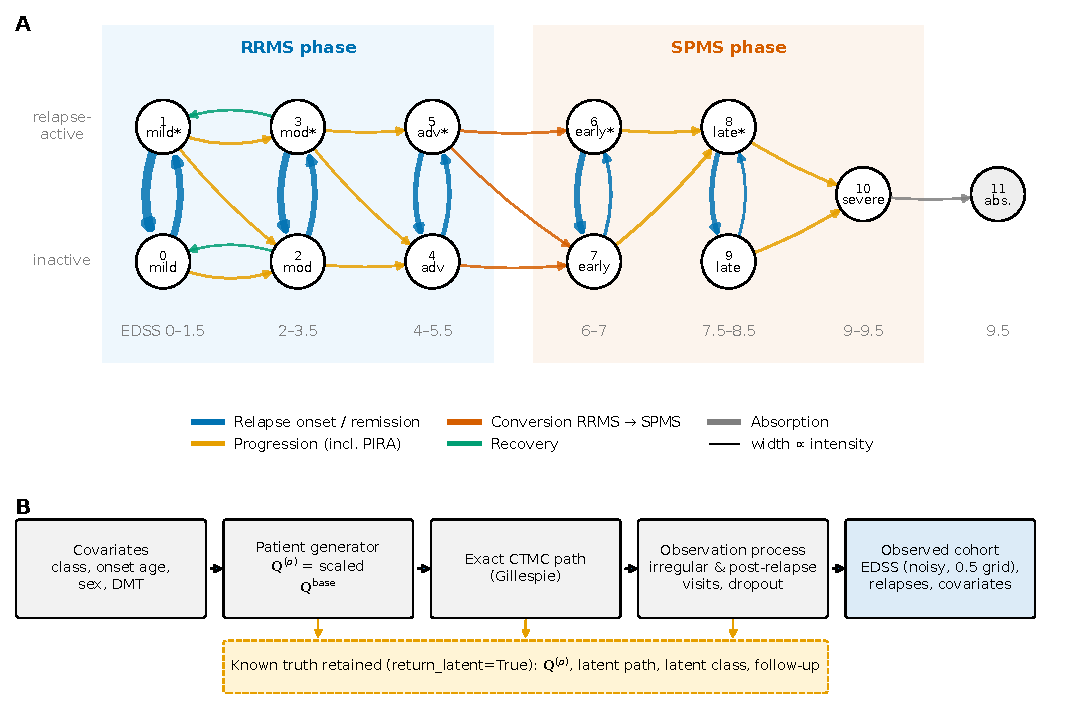
\includegraphics[width=\textwidth]{figs/fig1_model_structure.pdf}
\caption{Structure of the generator. \textbf{(A)} State-transition graph of $\Q^{\mathrm{base}}$. Nodes are the 12 macrostates arranged by EDSS band (horizontal) and relapse activity (vertical; asterisks mark relapse-active states); edge width is proportional to the transition intensity and colour to the edge type that determines covariate scaling. \textbf{(B)} Data-generating pipeline. The observed cohort is produced by the upper chain; the lower box lists the ground truth returned with it.}
\label{fig:model}
\end{figure}

\subsection*{A reference cohort reproduces natural-history benchmarks}

We generated a reference cohort of 500 patients with seed 42 and the default configuration. Unless stated otherwise, all statistics below refer to this cohort and are reproduced exactly by the repository (see Reproducibility). Definitions are given in Methods.

\paragraph{Cohort composition and observation structure.}
The cohort comprises 14,637 visit records: 29.3 visits per patient on average (median 34) over a median follow-up of 19.2 years (range 1.8--20.0). Inter-visit intervals average 6.45 months (median 5.96, SD 3.76), somewhat more frequent than the 1.3--1.6 annual visits reported in Big MS Data cohorts \cite{signori2023}, reflecting the configured 7-month RRMS interval and the additional relapse-triggered visits. Sex ratio and onset age match published cohorts closely (\cref{tab:descriptive}). Mean onset age is 1--3 years later than in London Ontario, Lyon and British Columbia \cite{scalfari2010,confavreux2006,palace2014}, and the mean EDSS slope of 0.15 points per year is close to the 0.11--0.13 reported for relapse-onset patients in MSBase \cite{ribbons2015}. \Cref{fig:trajectories} shows the latent path and the observed data of one representative patient from each latent class: measurement error scatters the observed EDSS around the band-level latent state, and short relapse episodes are recorded only when a visit falls close to them. \Cref{fig:realism} summarises the cohort-level distributions.

\begin{table}[htbp]
\centering
\caption{Reference cohort (N = 500, seed 42) compared with traceable published values. The synthetic cohort includes 80\% treated patients, whereas the London Ontario and AFFIRM placebo values describe untreated patients. ARR: annualised relapse rate (pooled person-time).}
\label{tab:descriptive}
\small
\begin{tabular}{p{5.2cm}p{3.1cm}p{6.4cm}}
\toprule
\textbf{Quantity} & \textbf{Synthetic} & \textbf{Published (source)}\\
\midrule
Female & 66.4\% & 66.0--74.2\% (Lyon, London Ontario, BCMS, Big MS Data) \cite{confavreux2006,scalfari2010,palace2014,signori2023}\\
Onset age, mean $\pm$ SD (years) & $31.7 \pm 8.8$ & 28.5--30.5 (London Ontario, Lyon, BCMS, UK RSS) \cite{scalfari2010,confavreux2006,palace2014}\\
Visits per year (12 / mean interval) & 1.86 (6.45 mo) & median 1.31--1.63 (Big MS Data) \cite{signori2023}\\
Baseline / last-visit EDSS, mean & 1.68 / 3.94 & --\\
EDSS slope, mean (median), points/yr & 0.151 (0.115) & 0.112 (women), 0.133 (men) (MSBase) \cite{ribbons2015}\\
Positive slope / slope $>0.5$ points/yr & 73.6\% / 7.6\% & --\\
ARR, RRMS phase (all patients) & 0.396 & 0.65 (London Ontario, untreated) \cite{scalfari2010}\\
ARR, untreated patients & 0.528 & 0.81 (AFFIRM placebo arm) \cite{polman2006}\\
ARR, SPMS phase & 0.281 & 0.23, SD 0.34 (Big MS Data SPMS) \cite{signori2023}\\
Converted to SPMS during follow-up & 27.8\% & 35\% by study end (BCMS) \cite{koch2010}\\
\bottomrule
\end{tabular}
\end{table}

\begin{figure}[htbp]
\centering
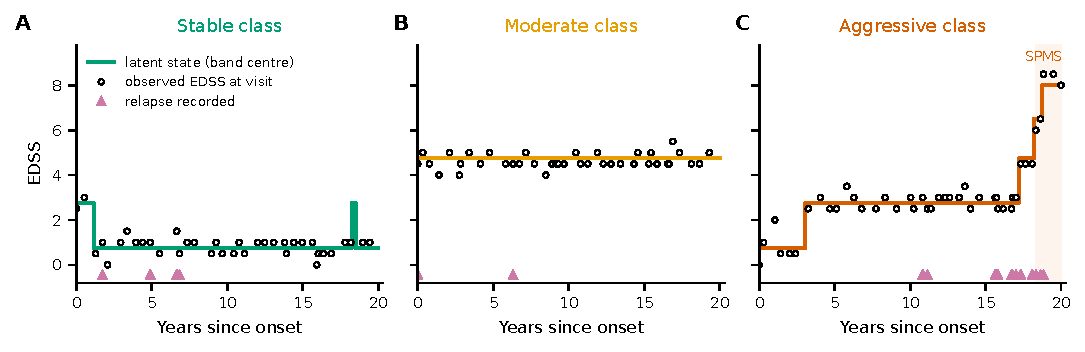
\includegraphics[width=\textwidth]{figs/fig2_latent_vs_observed.pdf}
\caption{Latent disease path and observed data for one representative patient per latent class (the patient with at least 15 years of follow-up whose last-visit EDSS is closest to the class median). Lines show the latent state (band centre), circles the observed EDSS at each visit, triangles recorded relapses; the shaded region marks the SPMS phase.}
\label{fig:trajectories}
\end{figure}

\begin{figure}[htbp]
\centering
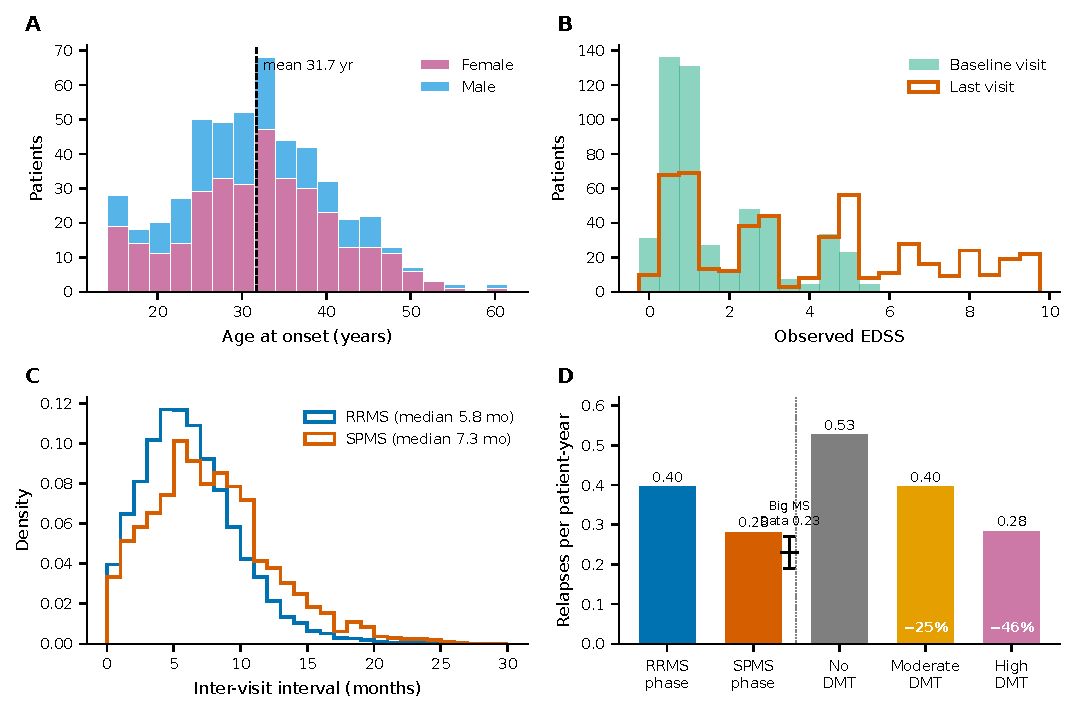
\includegraphics[width=\textwidth]{figs/fig3_cohort_realism.pdf}
\caption{Cohort-level characteristics of the reference cohort. \textbf{(A)} Onset age by sex. \textbf{(B)} Observed EDSS at the first and last visit. \textbf{(C)} Inter-visit intervals by the phase at the preceding visit. \textbf{(D)} Pooled annualised relapse rates by disease phase and by treatment; the black marker shows the Big MS Data SPMS-phase mean of 0.23 with the range of its trajectory-class means (0.19--0.27) \cite{signori2023}, and white labels give relative reductions versus untreated patients.}
\label{fig:realism}
\end{figure}

\paragraph{Relapse activity and treatment.}
Relapses occur at 0.396 per patient-year in the RRMS phase and 0.281 in the SPMS phase. These rates are lower than untreated natural-history rates because 80\% of the cohort is treated, and because relapses are only recorded when a visit falls within three months, which makes the observed rates conservative relative to the latent event rate. Among untreated patients the rate is 0.528, below the 0.65 of London Ontario \cite{scalfari2010} and the 0.81 of the AFFIRM placebo arm \cite{polman2006}. The SPMS-phase rate is above the Big MS Data mean of 0.23, but within its reported variability (SD 0.34) \cite{signori2023}. Relapse rates fall by 25.0\% with moderate-efficacy and 46.3\% with high-efficacy treatment (\cref{tab:dmt}). The high-efficacy value lies inside the 29--68\% range of reductions reported for licensed therapies \cite{mcginley2021} and close to network meta-analysis rate ratios of 0.28--0.42 for the most effective agents \cite{samjoo2023}; the moderate-efficacy value lies just below the lower end of that range.

\begin{table}[htbp]
\centering
\caption{Pooled annualised relapse rate by treatment status in the reference cohort.}
\label{tab:dmt}
\small
\begin{tabular}{lccc}
\toprule
\textbf{Treatment status} & \textbf{N (\%)} & \textbf{ARR (yr$^{-1}$)} & \textbf{Reduction vs untreated}\\
\midrule
None & 114 (22.8\%) & 0.528 & --\\
Moderate efficacy & 180 (36.0\%) & 0.396 & 25.0\%\\
High efficacy & 206 (41.2\%) & 0.284 & 46.3\%\\
\midrule
\multicolumn{4}{l}{Published: 29--68\% reduction vs placebo \cite{mcginley2021}; natalizumab 68\% (0.26 vs 0.81) \cite{polman2006}.}\\
\bottomrule
\end{tabular}
\end{table}

\paragraph{Disability accrual and conversion to SPMS.}
\Cref{tab:milestones} and \cref{fig:km} report Kaplan--Meier estimates of the time from onset to disability milestones. The cumulative probability of SPMS is 5.7\%, 17.8\%, 27.8\% and 37.0\% at 5, 10, 15 and 20 years; the median time to SPMS is not reached within 20 years. The medians for EDSS 6 and 8 are also not reached, whereas pre-treatment natural-history cohorts report medians of 15--21 years to SPMS and 18--23 years to EDSS 6 \cite{scalfari2010,leray2010,confavreux2006,koch2010}. Slower accrual in a predominantly treated cohort is the expected direction, and treatment is associated with a lower risk of conversion to SPMS in registry data \cite{brown2019}. The median time to EDSS 3 (8.4 years) is shorter than the 10 years reported in London Ontario and Rennes \cite{scalfari2010,leray2010}. Two definitional differences contribute (Methods): synthetic milestones are first-reached rather than confirmed, and 13.6\% of patients already have a true EDSS $\geq 3$ at their first visit.

The latent classes separate clearly. Kaplan--Meier SPMS probabilities at 10 and 20 years are 4.3\% and 8.4\% in the stable class (N = 143), 13.1\% and 34.0\% in the moderate class (N = 241) and 42.8\% and 74.6\% in the aggressive class (N = 116). Mean EDSS at the last visit is 2.12, 3.85 and 6.36, respectively. Seven trajectory classes were identified in a recent Swedish cohort \cite{guo2026} and three in SPMS patients from Big MS Data \cite{signori2023}; the three-class structure here is a design choice that recovery methods can be tested against.

\begin{table}[htbp]
\centering
\caption{Time from onset to disability milestones in the reference cohort (Kaplan--Meier) and published medians from untreated natural-history cohorts. Synthetic milestones are first-reached, unconfirmed values of true EDSS at a visit; published milestones are confirmed or irreversible. NR: median not reached within 20 years.}
\label{tab:milestones}
\small
\begin{tabular}{lccp{6.6cm}}
\toprule
\textbf{Milestone} & \textbf{Median (yr)} & \textbf{Cumulative 10 / 20 yr} & \textbf{Published median, years (cohort)}\\
\midrule
EDSS 3 & 8.4 & 55.0\% / 69.8\% & 10 (London Ontario) \cite{scalfari2010}; 10.0 (Rennes) \cite{leray2010}\\
EDSS 6 & NR & 17.8\% / 37.0\% & 18 (London Ontario); 21.7 (Rennes); 23.1 (Lyon) \cite{scalfari2010,leray2010,confavreux2006}\\
EDSS 8 & NR & 6.0\% / 23.3\% & 28 (London Ontario) \cite{scalfari2010}\\
SPMS & NR & 17.8\% / 37.0\% & 15 (London Ontario); 16.0 (Rennes); 21.4 (BCMS) \cite{scalfari2010,leray2010,koch2010}\\
\bottomrule
\end{tabular}
\end{table}

\begin{figure}[htbp]
\centering
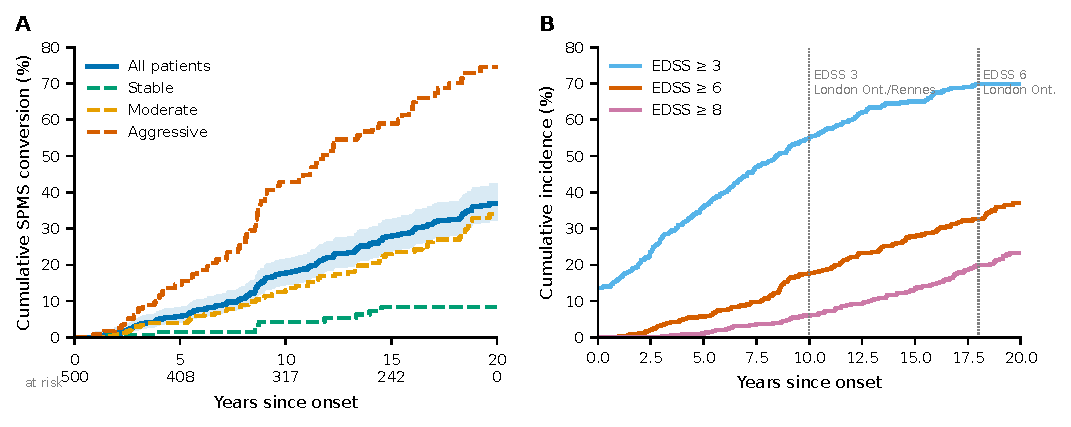
\includegraphics[width=\textwidth]{figs/fig4_kaplan_meier.pdf}
\caption{Kaplan--Meier estimates for the reference cohort. \textbf{(A)} Cumulative conversion to SPMS for all patients (95\% confidence band) and by latent class; numbers at risk are shown under the time axis. \textbf{(B)} Cumulative incidence of first reaching EDSS 3, 6 and 8; dotted lines mark published medians for EDSS 3 and EDSS 6 in London Ontario and Rennes \cite{scalfari2010,leray2010}. The EDSS 6 curve coincides with the all-patient SPMS curve in (A) by construction.}
\label{fig:km}
\end{figure}

\paragraph{Prognostic structure.}
Cox models for time to SPMS recover the directions built into the generator. The hazard ratio per standard deviation of onset age is 1.24 (95\% CI 1.05--1.46, $p=0.010$), per standard deviation of baseline EDSS 1.59 (1.36--1.85, $p<0.001$) and for male sex 1.34 (0.94--1.90, $p=0.10$), jointly adjusted. In univariable models each relapse in the first two years increases the hazard by 22\% (HR 1.22, 1.06--1.40, $p=0.005$), whereas any versus no early relapse is not associated with conversion (HR 0.97, 0.67--1.40). The sex effect is directionally correct but not significant at N = 500; the generator's modest built-in multiplier (1.15 on progression intensities) is small relative to the sampling variability of a cohort this size. Because the true multipliers are known, the power of a planned study to detect such effects can be estimated by simulation before real data are requested.

\subsection*{Known truth exposes estimator bias under registry-like observation}

The ground truth makes it possible to measure how well a method recovers the disease process from visit-level data. We illustrate this with the most basic task: estimating the generator matrix. Following the ADEMP framework for simulation studies \cite{morris2019}, we compared three estimators of the 26 non-zero intensities of $\Q^{\mathrm{base}}$ (Methods). The \emph{crude} estimator divides the number of visit-to-visit transitions from $i$ to $j$ by the time at risk in $i$; it is the maximum-likelihood estimator for continuously observed paths and is widely used as a shortcut for panel data. The \emph{panel} estimator maximises the panel likelihood $\prod \exp(\Q\,\Delta t)_{s_k s_{k+1}}$ over consecutive visits \cite{kalbfleisch1985,jackson2011}, with the structural zeros of $\Q$ known. The \emph{oracle} applies the crude formula to the exact latent paths and serves as an upper bound on attainable accuracy. We varied cohort size (250--4,000 patients), population heterogeneity (all patient-level scaling switched on or off), the visit process (relapse-triggered visits on or off) and visit frequency (mean intervals halved or doubled), with five independent replicates per design: 85 cohorts and 255 fits in total. \Cref{fig:benchmark} and \cref{tab:benchmark} summarise the results; all cells are listed in Additional file 1, Table S2.

\begin{table}[htbp]
\centering
\caption{Recovery of the 26 generating intensities by three estimators. Entries are the mean relative bias (\%) across intensities $\pm$ 1.96 Monte Carlo standard errors over five replicates, and the mean absolute relative error. In homogeneous populations every patient's generator equals $\Q^{\mathrm{base}}$; heterogeneous populations use the full patient-level scaling of \cref{eq:scaling}.}
\label{tab:benchmark}
\small
\begin{tabular}{p{4.6cm}rcccccc}
\toprule
& & \multicolumn{2}{c}{\textbf{Crude}} & \multicolumn{2}{c}{\textbf{Panel likelihood}} & \multicolumn{2}{c}{\textbf{Oracle}}\\
\cmidrule(lr){3-4}\cmidrule(lr){5-6}\cmidrule(lr){7-8}
\textbf{Design} & \textbf{N} & Bias (\%) & $|$err$|$ & Bias (\%) & $|$err$|$ & Bias (\%) & $|$err$|$\\
\midrule
Homogeneous, non-informative visits & 250 & $-19.6\pm1.5$ & 0.289 & $+1.4\pm2.7$ & 0.212 & $+1.8\pm2.4$ & 0.172 \\
 & 4000 & $-21.0\pm1.1$ & 0.245 & $+0.1\pm0.8$ & 0.049 & $+0.3\pm0.5$ & 0.038 \\
\addlinespace
Homogeneous, relapse-triggered visits & 250 & $-13.4\pm3.9$ & 0.241 & $+9.2\pm6.4$ & 0.274 & $+2.1\pm5.6$ & 0.164 \\
 & 4000 & $-14.7\pm1.2$ & 0.158 & $+5.8\pm1.2$ & 0.131 & $0.0\pm1.2$ & 0.037 \\
\addlinespace
Heterogeneous, relapse-triggered visits & 250 & $-20.3\pm3.9$ & 0.352 & $-6.7\pm4.9$ & 0.317 & $-8.8\pm4.2$ & 0.308 \\
 & 4000 & $-20.6\pm1.2$ & 0.310 & $-8.3\pm1.4$ & 0.237 & $-10.1\pm1.3$ & 0.240 \\
\addlinespace
Visit interval $\times$0.5 (non-inform.) & 1000 & $-12.8\pm2.8$ & 0.185 & $-0.1\pm2.9$ & 0.103 & $0.0\pm2.3$ & 0.087 \\
Visit interval $\times$1 (non-inform.) & 1000 & $-21.4\pm1.6$ & 0.260 & $0.0\pm1.8$ & 0.104 & $+0.6\pm1.4$ & 0.087 \\
Visit interval $\times$2 (non-inform.) & 1000 & $-33.4\pm3.0$ & 0.387 & $-0.3\pm3.3$ & 0.125 & $-0.6\pm2.6$ & 0.076 \\
\bottomrule
\end{tabular}
\end{table}

\paragraph{The crude estimator is biased, and more data do not help.}
With non-informative visits in a homogeneous population, the crude estimator underestimated the intensities on average: its mean bias was $-19.6\%$ at N = 250 and $-21.0\%$ at N = 4,000: the bias does not shrink with cohort size, so its error reaches a floor of about 0.25. The bias is concentrated in the fast, reversible relapse and remission transitions (\cref{fig:benchmark}A), where several jumps can occur between consecutive visits and the crude estimator records none, one, or a net change. It grows with visit spacing, from $-12.8\%$ with 3.5-month intervals to $-21.4\%$ at the default 7 months and $-33.4\%$ at 14 months (\cref{fig:benchmark}E).

\paragraph{The panel likelihood is unbiased only if visits are non-informative.}
Under non-informative visits the panel estimator was unbiased at every cohort size and visit frequency (bias within $\pm1.4\%$), and its error fell from 0.21 to 0.05 as N increased sixteen-fold, close to the oracle's decline from 0.17 to 0.04 and consistent with $N^{-1/2}$ convergence. When visits followed relapses, the panel estimator overestimated the intensities by $+5.8\% \pm 1.2\%$ at N = 4,000, and this bias did not decrease with cohort size (\cref{fig:benchmark}B,C). A plausible mechanism is that relapse-triggered visits sample the path shortly after entry into a relapse-active state, so that observed pairs over-represent short sojourns, which a likelihood that assumes path-independent visit times explains by higher intensities. The crude estimator's bias was smaller in this setting ($-14.7\%$); consistent with the visit-frequency results, the additional closely spaced visits partly offset its under-counting. These results illustrate the general problem of informative observation times in multi-state models \cite{lange2015}: a standard estimator can be precise, apparently well behaved, and still converge to the wrong value. Such bias is invisible in real data because the true intensities are unknown.

\paragraph{Heterogeneity changes the estimand.}
When class, age, sex and treatment scaling are active, no pooled estimator converges to $\Q^{\mathrm{base}}$. Even the oracle had a mean bias of $-10.1\%$ and an error of 0.24 at N = 4,000, because a pooled estimate targets an exposure-weighted average of patient-specific generators rather than any single patient's (\cref{fig:benchmark}D). The same two effects operate in the reference cohort: the oracle, which is free of observation error, already has a mean error of 0.25 with respect to $\Q^{\mathrm{base}}$, and the crude estimator adds a systematic bias of $-18\%$ from panel observation, giving a mean error of 0.31 (\cref{fig:benchmark}F; per-transition values in Additional file 1, Table S1). Methods that model heterogeneity, such as covariate-dependent or latent-class multi-state models, can be evaluated against the patient-level generators that ms-synth returns.

\paragraph{Computation.}
The crude and oracle estimators take under 0.4 s at N = 4,000. The vectorised panel likelihood takes a median of 1.7 s at N = 250 and 29 s at N = 4,000 (103,000--120,000 visits) on one core. Each likelihood evaluation is about 35 times faster than computing one matrix exponential per visit pair, and the two implementations agree to $10^{-15}$.

\begin{figure}[htbp]
\centering
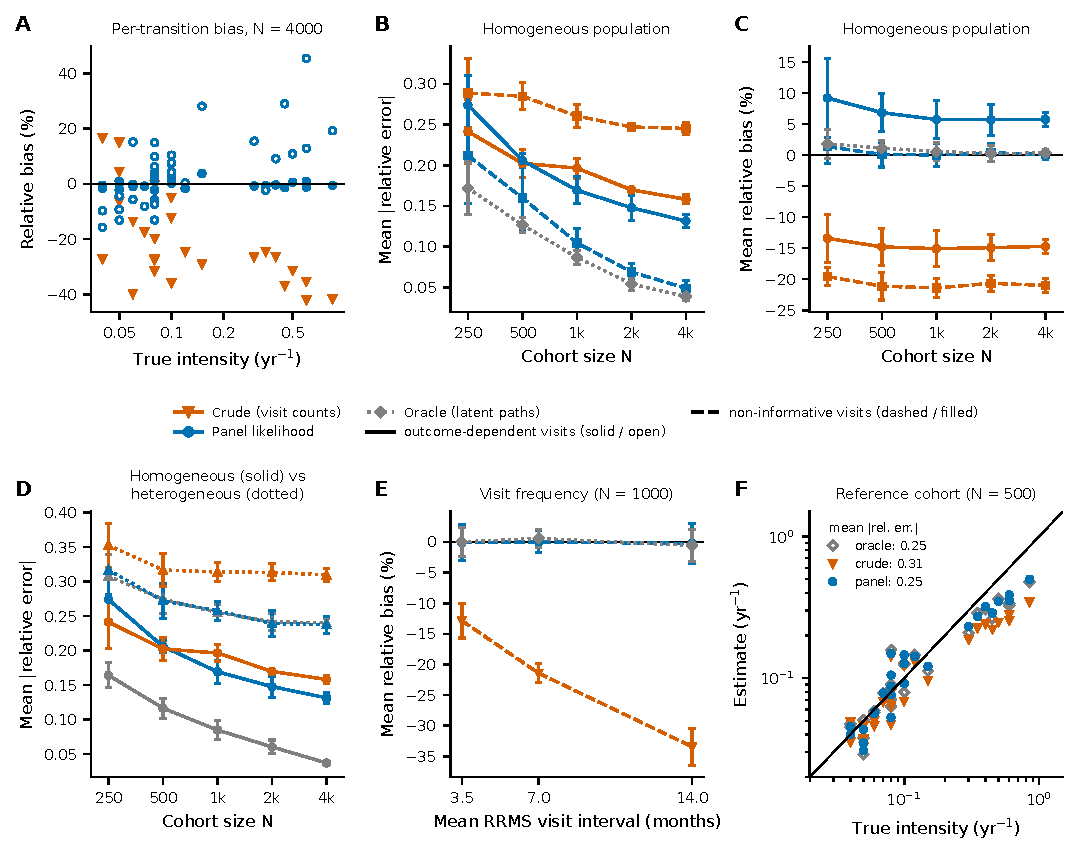
\includegraphics[width=\textwidth]{figs/fig5_estimator_benchmark.pdf}
\caption{Known-truth benchmark of generator-matrix estimators. \textbf{(A)} Relative bias of each of the 26 intensities at N = 4,000 (homogeneous population, mean of five replicates) against the true intensity: crude estimator (triangles) and panel likelihood under non-informative (filled circles) and relapse-triggered visits (open circles). \textbf{(B, C)} Mean absolute relative error and mean relative bias against cohort size; solid lines, relapse-triggered visits; dashed lines, non-informative visits; dotted, oracle. \textbf{(D)} Error against cohort size in homogeneous (solid) and heterogeneous (dotted) populations. \textbf{(E)} Bias against mean visit interval at N = 1,000 with non-informative visits. \textbf{(F)} True against estimated intensities in the reference cohort (N = 500, seed 42). Error bars are 1.96 Monte Carlo standard errors.}
\label{fig:benchmark}
\end{figure}

\subsection*{Reproducibility}

Every result in this article can be regenerated from version 1.0.0 of the repository \cite{mssynth} with a single command (\soft{bash reproduce.sh}), which installs the exact dependency versions from a lock file, runs the test suite, recomputes all statistics, reruns the estimator benchmark and redraws all figures. A verification script regenerates the reference cohort, compares its SHA-256 checksum with a stored value, and compares every reported statistic with a stored reference file. The benchmark checkpoints each replicate so that interrupted runs resume. With Python 3.12, the reference cohort file was byte-identical under two software stacks (NumPy 2.4.4, SciPy 1.17.1, pandas 3.0.2 and NumPy 2.5.3, SciPy 1.18.1, pandas 2.3.3). Across NumPy 2.4.4/2.5.3 and SciPy 1.17.1/1.18.1, every derived statistic was identical except the panel-likelihood estimates, which differed in the fourth decimal because of optimiser termination; the verification tolerates differences up to $10^{-3}$ for these values only. Software versions are pinned, a citation file is provided \cite{smith2016}, a continuous-integration workflow is configured to run the tests on three operating systems and four Python versions, and the benchmark takes about 15 minutes on one core. These practices follow published recommendations for reproducible computational research \cite{sandve2013,wilkinson2016}.

%% =================================================================== DISCUSSION
\section*{Discussion}
\addcontentsline{toc}{section}{Discussion}

ms-synth generates synthetic MS cohorts whose data-generating process is fully known and whose observation process has the features that complicate analysis of real registry data: irregular visits, visits triggered by relapses, noisy half-point EDSS scores and censoring. A reference cohort reproduces the sex ratio, onset age, relapse rates, treatment effects, EDSS slopes and milestone timing reported by natural-history cohorts, registries and trials, within the deviations documented below. The estimator benchmark shows what this combination makes possible. A simple and widely used estimator is biased by about 20\%, and the bias worsens with sparser visits. The standard panel likelihood is unbiased only when visit times are unrelated to the disease path. Heterogeneity between patients means that a pooled estimate does not describe any individual patient. None of these problems can be detected in real data, where the truth is unknown, and each has practical consequences for published multi-state analyses of MS registries.

\paragraph{Intended uses.}
The generator is not tied to a particular analysis. For multi-state and panel-data methods it provides a test bed in which misclassification models, covariate effects and joint models of disease and visit processes \cite{lange2015} can be scored against the true patient generators; the switch between informative and non-informative visits makes the benefit of such joint models measurable. For survival and milestone analyses it supplies exact event times alongside interval-censored, visit-based observations, so that confirmation rules, censoring assumptions and the handling of events present at the first visit can be assessed. For trajectory clustering and latent-class models \cite{signori2023,guo2026} the true class of every patient is known. For the percolation analysis that motivated the project \cite{mirkov2026}, the known $\Q$ allows three checks: whether the critical threshold estimated from a fitted $\Q$ matches that of the generating matrix; whether class-specific generators produce distinguishable percolation curves; and whether patient-level distances to the threshold anticipate conversion to SPMS. More generally, the generator lets analysis pipelines be built and tested before registry data are requested, and it can be used in teaching.

\paragraph{Calibration relative to published cohorts.}
Agreement with published values is close for sex ratio, visit frequency, EDSS slope and relapse reduction under high-efficacy treatment. Five deviations are documented, and each is controlled by one configuration parameter.
\begin{enumerate}[leftmargin=*,itemsep=1pt,topsep=2pt]
\item Onset age is 1--3 years later than in London Ontario, Lyon and British Columbia; the configured mean of 32 years can be lowered to 30.
\item Time to EDSS 3 is shorter than published, partly for the definitional reasons discussed above and partly because 35\% of patients start with EDSS $\geq 2$. This is governed by the onset-state distribution and the progression intensities out of the mild and moderate RRMS states.
\item The relapse rate of untreated patients (0.53) is below natural-history values (0.65--0.81). One reason is that relapses are observed only within three months of a visit; the relapse-onset intensities can be raised.
\item The SPMS-phase relapse rate is slightly higher than the Big MS Data mean; this is governed by the SPMS cycling intensities.
\item The moderate-efficacy treatment effect (25\%) is just below the published range; a relapse multiplier of about 0.60 instead of 0.65 brings it inside.
\end{enumerate}
Disability milestones are reached more slowly than in untreated cohorts, as expected with 80\% treatment; setting all patients to untreated gives an untreated scenario, whose agreement with natural-history milestones we have not evaluated here. We report results for the unmodified configuration so that they are reproducible from a single seed, and we provide the verified compilation of published parameters in the repository so that users can recalibrate for their own purposes.

\paragraph{Limitations.}
The disease process is a time-homogeneous Markov chain. Sojourn times are exponential, intensities do not depend on disease duration or current age beyond the onset-age scaling, and treatment status is fixed for each patient, without switching or discontinuation. EDSS is represented at the resolution of bands, with continuous variation added only by the within-band noise model. Because every state with EDSS $\geq 6$ belongs to SPMS, EDSS 6 and SPMS cannot be distinguished. Primary progressive MS is not represented. The intensities were calibrated by hand to aggregate targets rather than by formal methods such as approximate Bayesian computation or history matching, and the reference configuration is one plausible parameter set rather than an estimate for any real population. The EDSS milestones are unconfirmed, whereas clinical definitions require confirmation over 3--6 months. Finally, results obtained on synthetic data show whether a method can recover a known process under realistic conditions; they do not replace validation of clinical conclusions on real data.

\paragraph{Future development.}
Planned extensions include formal calibration against the compiled natural-history targets, time-varying and duration-dependent intensities, treatment switching, a primary progressive branch, confirmed-disability definitions, and built-in estimators that model the visit process jointly with the disease process.

\section*{Conclusions}
\addcontentsline{toc}{section}{Conclusions}

ms-synth makes the validation of MS progression methods possible without restricted data and without guessing at the truth. Its reference cohort matches traceable natural-history benchmarks, and its first application already shows that routine estimators of multi-state models can be substantially biased under registry-like observation. The software, reference outputs and verification tools are openly available and reproduce every result in this article.

%% =================================================================== METHODS
\section*{Methods}
\addcontentsline{toc}{section}{Methods}

\paragraph{Analysis of the reference cohort.}
The reference cohort was generated with seed 42, 500 patients and the default configuration. Follow-up is the time of the last visit. Time to SPMS is the time of the first visit whose latent state lies in the SPMS phase; patients without such a visit are censored at their last visit. Time to EDSS $k$ ($k=3,6,8$) is the time of the first visit with true EDSS $\geq k$, without confirmation, and events at the first visit are included (13.6\% of patients for EDSS 3). Survival functions were estimated with the Kaplan--Meier method and log--log confidence intervals \cite{davidsonpilon2019}. Annualised relapse rates are pooled over person-time: recorded relapses divided by follow-up time in the stratum, with phase-specific person-time split at the first SPMS visit. The EDSS slope is the ordinary least-squares slope of observed EDSS on time since onset. A slope counts as positive only if it exceeds $10^{-9}$ points per year: a numerically flat trajectory has a fitted slope of about $10^{-16}$ whose sign depends on the linear-algebra library, and without the tolerance the percentage of positive slopes differed between platforms (73.6\% versus 73.8\%). Cox proportional-hazards models for time to SPMS used, in turn, an indicator of any recorded relapse in the first two years, the number of such relapses, and a joint model of onset age and baseline EDSS (both standardised) and male sex.

\paragraph{Estimator benchmark.}
The benchmark follows the ADEMP structure \cite{morris2019}. \emph{Data-generating mechanisms}: (A) cohort sizes of 250, 500, 1,000, 2,000 and 4,000 patients, in homogeneous and heterogeneous populations, with the default relapse-triggered visits; (B) 1,000 patients, homogeneous population, non-informative visits, with both mean visit intervals multiplied by 0.5 or 2; (C) the five cohort sizes, homogeneous population, non-informative visits. In homogeneous populations all patients belong to the moderate class (multipliers of 1), the age and sex multipliers are set to 1 and nobody is treated, so every patient generator equals $\Q^{\mathrm{base}}$. Non-informative visits are obtained by switching off the relapse-triggered visit. Each design was replicated with seeds 1000--1004. \emph{Estimands}: the 26 non-zero intensities of $\Q^{\mathrm{base}}$. \emph{Methods}: with $N_{ij}$ the number of consecutive visit pairs in states $(i,j)$ and $T_i$ the summed intervals of pairs starting in $i$, the crude estimator is $\hat\lambda_{ij}=N_{ij}/T_i$. The panel estimator maximises $\sum_k \log[\exp(\Q\,\Delta t_k)]_{s_k s_{k+1}}$ over the logarithms of the 26 intensities with L-BFGS-B, starting from the crude estimate (floored at $10^{-3}$), without penalty. Transition probabilities are computed from the eigendecomposition of $\Q$, with a batched matrix exponential used when the eigenvector matrix is ill-conditioned (condition number $>10^{8}$). The oracle applies $N_{ij}/T_i$ to the exact latent paths truncated at each patient's follow-up. \emph{Performance measures}: for each replicate, the mean relative bias $(\hat\lambda-\lambda)/\lambda$ and the mean absolute relative error over the 26 intensities; these were averaged over replicates, and Monte Carlo standard errors were computed as the standard deviation across replicates divided by $\sqrt{5}$.

\paragraph{Software and computing environment.}
All results were produced with ms-synth 1.0.0 under Python 3.12.3 with NumPy 2.5.3, SciPy 1.18.1, pandas 2.3.3, lifelines 0.30.3 and Matplotlib 3.11.2 \cite{harris2020,virtanen2020,mckinney2010,davidsonpilon2019,hunter2007}, on a single core of an Intel Xeon processor (2.1 GHz). The complete environment is pinned in \soft{requirements-lock.txt}.

%% =================================================================== BACK MATTER
\section*{Availability of supporting source code and requirements}
\addcontentsline{toc}{section}{Availability of supporting source code and requirements}
\begin{itemize}[leftmargin=*,itemsep=0pt]
\item Project name: ms-synth
\item Project home page: \url{https://github.com/nikola-m/ms-synth}
\item Version: 1.0.0 (archived snapshot: Zenodo DOI [to be assigned at release])
\item Operating system(s): Platform independent
\item Programming language: Python
\item Other requirements: Python $\geq$ 3.10; NumPy, SciPy, pandas, PyYAML; optional lifelines and Matplotlib (analyses and figures), NetworkX (percolation module)
\item License: MIT
\item RRID: [to be registered at SciCrunch]
\item bio.tools ID: [to be registered]
\end{itemize}

\section*{Data availability}
\addcontentsline{toc}{section}{Data availability}
No real patient data were used. The reference cohort (N = 500, seed 42) is regenerated byte-identically by \soft{make cohort}, and its SHA-256 checksum, the expected values of all reported statistics, the raw and summarised benchmark estimates and the figure source data are provided in the \soft{reference/} and \soft{results/} directories of the repository \cite{mssynth}. The compilation of published natural-history parameters used for calibration is provided as \soft{Validation.md}. An archival copy of the code and supporting data will be deposited in the GigaScience repository, GigaDB, on acceptance. Additional file 1 contains Tables S1--S3.

\section*{Abbreviations}
\addcontentsline{toc}{section}{Abbreviations}
ADEMP: aims, data-generating mechanisms, estimands, methods and performance measures; ARR: annualised relapse rate; BCMS: British Columbia Multiple Sclerosis database; CI: confidence interval; CSV: comma-separated values; EDSS: Expanded Disability Status Scale; EHR: electronic health record; HR: hazard ratio; MS: multiple sclerosis; PIRA: progression independent of relapse activity; RRMS: relapsing--remitting multiple sclerosis; SD: standard deviation; SPMS: secondary progressive multiple sclerosis; UK RSS: UK multiple sclerosis risk-sharing scheme; YAML: YAML Ain't Markup Language (configuration format).

\section*{Declarations}
\addcontentsline{toc}{section}{Declarations}
\paragraph{Ethics approval and consent to participate.} Not applicable. The study uses only synthetic data generated by software and involves no human participants or human data.
\paragraph{Consent for publication.} Not applicable.
\paragraph{Competing interests.} The authors declare that they have no competing interests.
\paragraph{Funding.} No external funding was received for this work.
\paragraph{Authors' contributions.} All authors contributed to conceptualisation, methodology, software development and manuscript writing. [To be completed with individual CRediT roles, as recommended by the journal.]
\paragraph{Acknowledgements.} [To be completed by the authors, including the disclosure of any use of generative AI tools in code or manuscript preparation, with tool, model version, dates and user, as required by the journal.]

\bibliographystyle{unsrtnat}
\bibliography{references}

\end{document}
